\chapter{Resultados e Conclusões}
\noindent

	Neste capítulo serão apresentados os parâmetros utilizados nas simulações e os resultados obtidos para cada caso. Ainda, uma análise de erro é efetivada para a verificação da ordem do método. Todas as simulações foram feitas até o tempo de $20$ segundos para os CFL's indicados.
	
	Vale lembrar que as funções utilizadas para a difusão unidimensional e bidimensional e para a advecção unidimensional e bidimensional são aquelas dadas pelas Eq.(\ref{difused}), Eq.(\ref{difused2}), Eq.(\ref{soladvuni}) e Eq.(\ref{soladvbi}), respectivamente.
		
\section{Difusão Unidimensional}
\noindent

	Para o caso da difusão unidimensional, faz-se uma simulação numérica com diferentes números de divisões espaciais em uma dimensão para avaliar a convergência e o refinamento do resultado com a diminuição dos intervalos no espaço e, consequentemente, no tempo. Para o método explícito na difusão, o CFL limite é de $1/2$, sendo que para valores maiores que esse a simulação diverge.
	
	Ainda, espera-se para este caso explícito, como dado pela Eq.(\ref{expeight}), um erro de segunda ordem. Ou seja, ao reduzir o intervalo diferencial $\Delta x$ para metade de seu valor inicial, o erro deve reduzir quatro vezes. Verifica-se que tal evento é confirmado na Tabela(\ref{tabela1}).

\begin{table}[h!]
	\caption{Erro do método numérico do caso explícito para $CFL$=0,5.}
	\label{tabela1}
	\centering
	\begin{tabular}{c | c c c | c c c}
		\hline
		Número de nós  espaciais&       Erro $L_\infty$       	& Razão   	 & Ordem   & Erro $L_{2}$ 				& Razão 	  & Ordem  \\ \hline
		$50$ 					&		$2,31 \, . 10^{-5}$     & $---$      & $---$   &       $1,62 \, . 10^{-5}$  & $---$       & $---$    \\ 
		$100$ 					&       $5,66 \, . 10^{-6}$     & $4,08$     & $2,03$  &       $3,98 \, . 10^{-6}$  & $4,06$      & $2,02$    \\ 
		$200$ 					&       $1,40 \, . 10^{-6}$     & $4,04$     & $2,01$  &       $9,87 \, . 10^{-7}$  & $4,03$      & $2,01$    \\ 
		$400$ 					&       $3,48 \, . 10^{-7}$     & $4.02$     & $2.01$  &       $2,46 \, . 10^{-7}$  & $4,01$      & $2,01$    \\ \hline
	\end{tabular}
\end{table}

	Assim como para o método explícito, o método implícito para a difusão unidimensional é um método de segunda ordem. Os valores obtidos são apresentados na Tabela(\ref{tabela2}).
	
\begin{table}[h!]
	\caption{Erro do método numérico do caso implícito para $CFL$=0,5.}
	\label{tabela2}
	\centering
	\begin{tabular}{c | c c c | c c c}
		\hline
		Número de nós  espaciais&       Erro $L_\infty$       	& Razão   	 & Ordem   & Erro $L_{2}$ 				& Razão 	  & Ordem  \\ \hline
		$50$ 					&		$1,01 \, . 10^{-3}$     & $---$      & $---$   &       $9,58 \, . 10^{-4}$  & $---$       & $---$    \\ 
		$100$ 					&       $2,47 \, . 10^{-4}$     & $4,07$     & $2,03$  &       $1,74 \, . 10^{-4}$  & $5,51$      & $2,75$    \\ 
		$200$ 					&       $6,11 \, . 10^{-5}$     & $4,04$     & $2,02$  &       $4,31 \, . 10^{-5}$  & $4,03$      & $2,01$    \\ 
		$400$ 					&       $1,50 \, . 10^{-5}$     & $4.06$     & $2.03$  &       $1,06 \, . 10^{-5}$  & $4,05$      & $2,02$    \\ \hline
	\end{tabular}
\end{table}

	É conveniente plotar as relações da resolução numérica e analítica para esse caso. A Figura(4.1) apresenta o gráfico para o método explícito, enquanto a Figura(4.2) apresenta o do método implícito.
	
\begin{figure}[ht!]
	\label{explicito1}
	\centering
	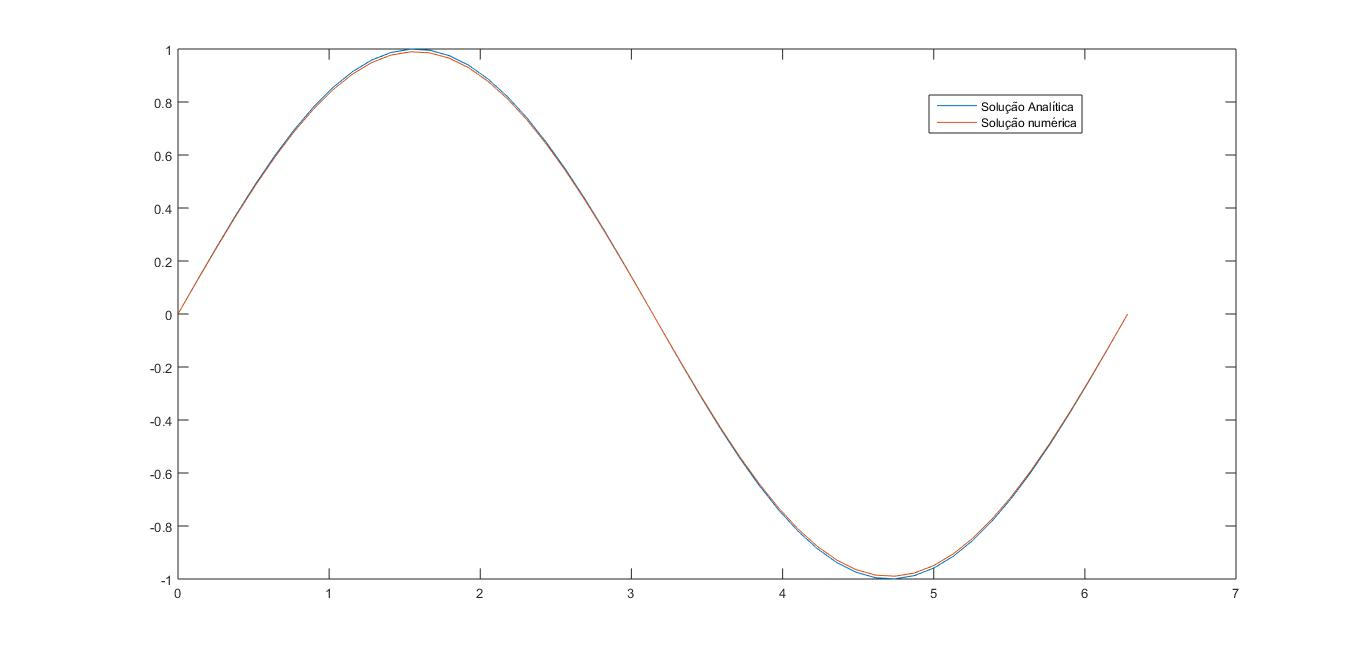
\includegraphics[width=135mm]{Imagens/uniexplicito.png}
	\caption{Difusão unidimensional pelo método explícito}
\end{figure}

\begin{figure}[ht!]
	\label{implicito1}
	\centering
	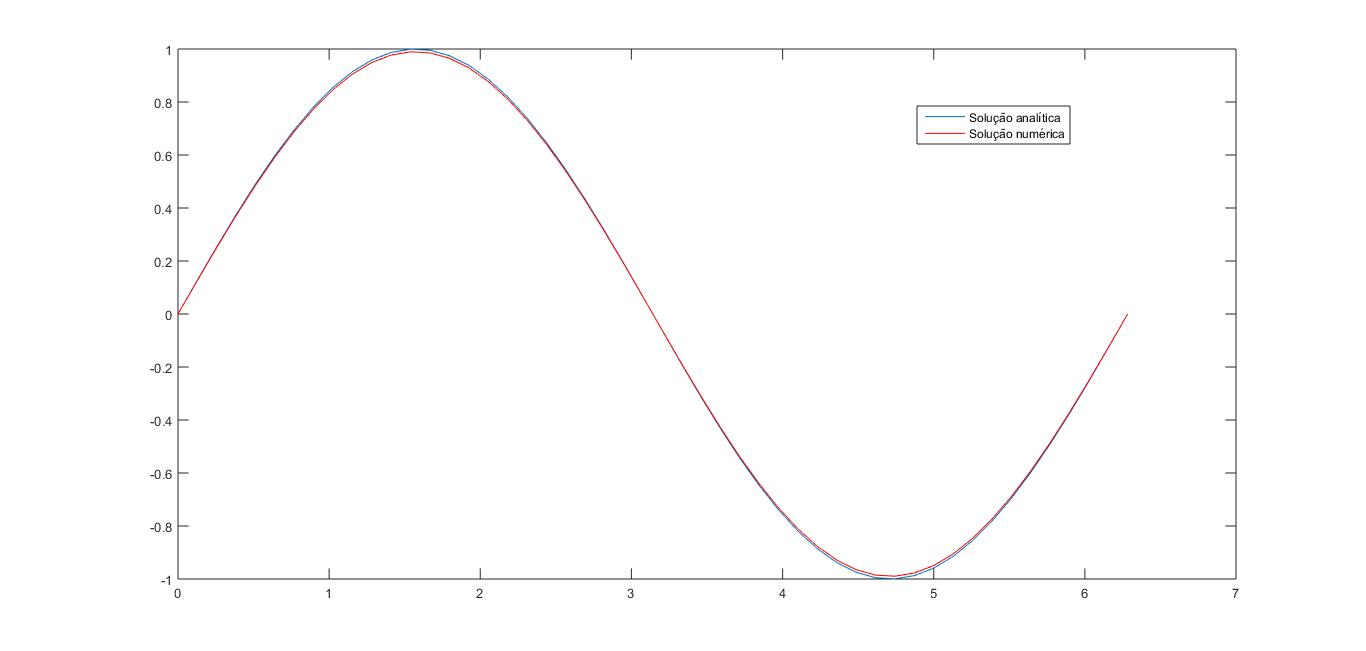
\includegraphics[width=135mm]{Imagens/uniimplicito.png}
	\caption{Difusão unidimensional pelo método implícito}
\end{figure}

\newpage
\section{Difusão Bidimensional}
\noindent

	Assim como no caso unidimensional, faz-se uma simulação numérica com diferentes números de divisões espaciais, agora nas duas dimensões, para avaliar a convergência e o refinamento do resultado com a diminuição dos intervalos no espaço e no tempo. O CFL limite continua sendo $1/2$ para garantir a convergência.
	
	A Tabela(\ref{tabela3}), dada a seguir, apresenta os resultados para os erros e a ordem para o método explícito, enquanto a Tabela(\ref{tabela4}) apresenta esses dados para o método implícito.
	
	\begin{table}[h!]
	\caption{Erro do método numérico do caso bidimensional explícito para $CFL$=0,5.}
	\label{tabela3}
	\centering
	\begin{tabular}{c | c c c | c c c}
		\hline
		Número de nós  espaciais&       Erro $L_\infty$       	& Razão   	 & Ordem   & Erro $L_{2}$ 				& Razão 	  & Ordem  \\ \hline
		$25$ 					&		$3,08 \, . 10^{-3}$     & $---$      & $---$   &       $1,48 \, . 10^{-3}$  & $---$       & $---$    \\ 
		$50$ 					&       $7,38 \, . 10^{-4}$     & $4,18$     & $2,09$  &       $3,62 \, . 10^{-4}$  & $4,08$      & $2,04$    \\ 
		$100$ 					&       $1,81 \, . 10^{-4}$     & $4,08$     & $2,04$  &       $8,96 \, . 10^{-5}$  & $4,04$      & $2,02$    \\ 
		$200$ 					&       $4,48 \, . 10^{-5}$     & $4.04$     & $2.02$  &       $2,23 \, . 10^{-5}$  & $4,02$      & $2,01$    \\ \hline
	\end{tabular}
\end{table}

	\begin{table}[h!]
	\caption{Erro do método numérico do caso bidimensional implícito para $CFL$=0,5.}
	\label{tabela4}
	\centering
	\begin{tabular}{c | c c c | c c c}
		\hline
		Número de nós  espaciais&       Erro $L_\infty$       	& Razão   	 & Ordem   & Erro $L_{2}$ 				& Razão 	  & Ordem  \\ \hline
		$25$ 					&		$1,49 \, . 10^{-3}$     & $---$      & $---$   &       $7,14 \, . 10^{-4}$  & $---$       & $---$    \\ 
		$50$ 					&       $3,56 \, . 10^{-4}$     & $4,18$     & $2,09$  &       $1,75 \, . 10^{-4}$  & $4,10$      & $2,05$    \\ 
		$100$ 					&       $8,73 \, . 10^{-5}$     & $4,08$     & $2,04$  &       $4,32 \, . 10^{-5}$  & $4,04$      & $2,02$    \\ 
		$200$ 					&       $5,37 \, . 10^{-5}$     & $4.04$     & $2.02$  &       $1,07 \, . 10^{-5}$  & $4,02$      & $2,01$    \\ \hline
	\end{tabular}
\end{table}

	As representações gráficas dos resultados numéricos para os métodos explícito e implícito são fornecidas pelas Figura(4.3) e Figura(4.4), respectivamente.

\newpage

\begin{figure}[ht!]
	\label{explicito2}
	\centering
	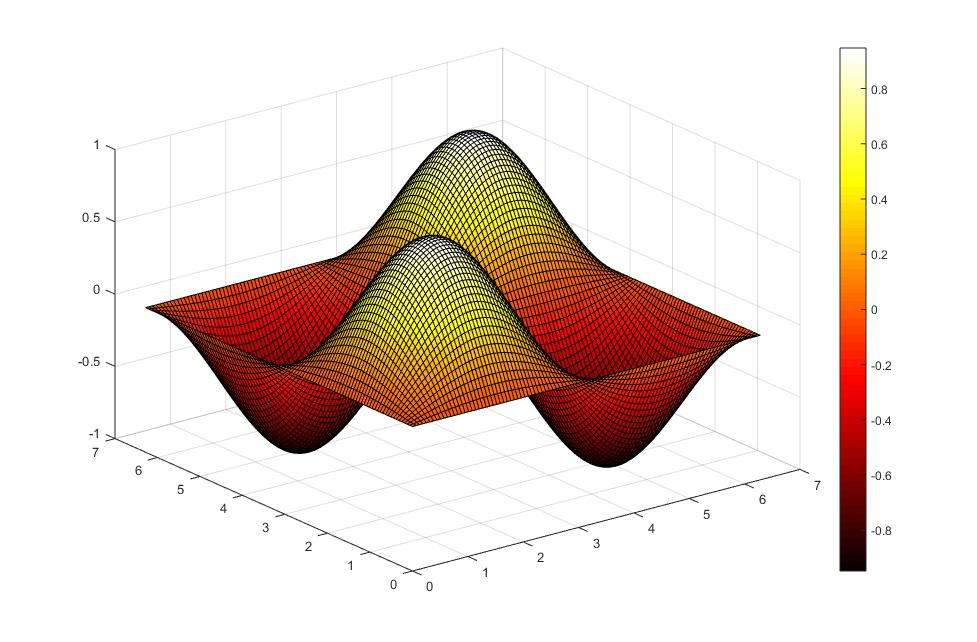
\includegraphics[width=140mm]{Imagens/biexplicito.png}
	\caption{Difusão bidimensional pelo método explícito}
\end{figure}

\begin{figure}[ht!]
	\label{implicito10}
	\centering
	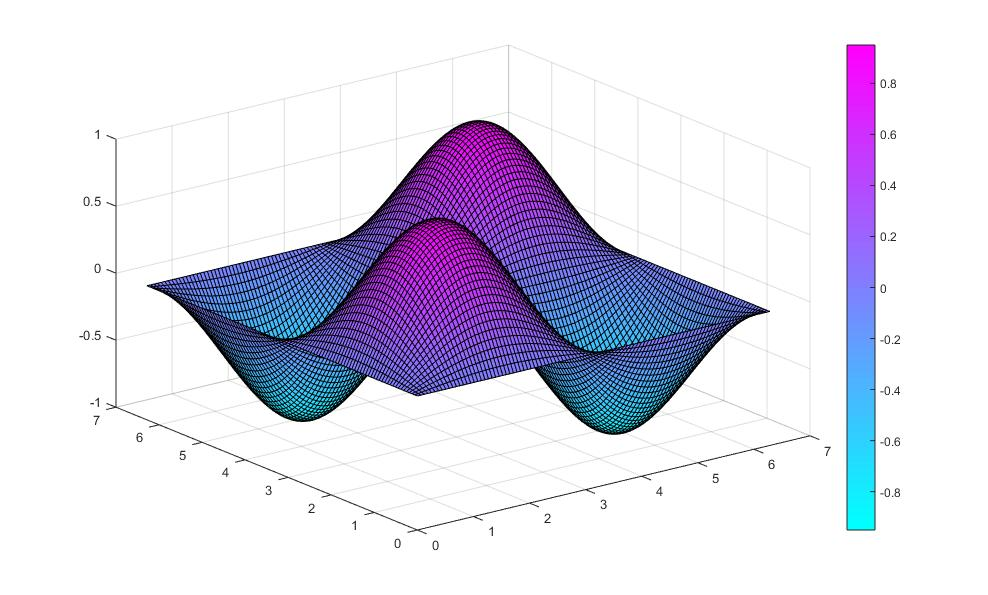
\includegraphics[width=140mm]{Imagens/biimplicito.png}
	\caption{Difusão bidimensional pelo método implícito}
\end{figure}

\newpage

\section{Advecção Unidimensional}
\noindent

	Repete-se aqui o procedimento utilizado para a difusão, sabendo agora que o método é de primeira ordem. A velocidade de advecção é definida como $-1 \ m/s$. Ainda, para o caso da advecção existe um CFL otimizado já conhecido para a solução. Para o CFL unitário, os erros chegam à ordem de $-15$, enquanto para $1/2$, os erros flutuam ao redor da ordem de $-2$. 
	
	Nota-se pela Figura(4.5) que informações são perdidas no decorrer das rotinas computacionais. Esse comportamento é característico de métodos de discretização difusivos, como é o caso para o upwind scheme de primeira ordem. 
	
	\begin{table}[h!]
	\caption{Erro do método numérico do caso unidimensional explícito para $CFL$=0,5.}
	\label{tabela5}
	\centering
	\begin{tabular}{c | c c c | c c c}
		\hline
		Número de nós  espaciais&       Erro $L_\infty$       	& Razão   	 & Ordem   & Erro $L_{2}$ 				& Razão 	  & Ordem  \\ \hline
		$50$ 					&		$1,70 \, . 10^{-1}$     & $---$      & $---$   &       $8,17 \, . 10^{-2}$  & $---$       & $---$    \\ 
		$100$ 					&       $8,89 \, . 10^{-2}$     & $1,91$     & $0,96$  &       $4,26 \, . 10^{-2}$  & $1,92$      & $0,96$    \\ 
		$200$ 					&       $4,56 \, . 10^{-2}$     & $1,95$     & $0,97$  &       $2,17 \, . 10^{-2}$  & $1,96$      & $0,98$    \\ 
		$400$ 					&       $2,31 \, . 10^{-2}$     & $1,98$     & $0,99$  &       $1,09 \, . 10^{-2}$  & $1,98$      & $0,99$    \\ \hline
	\end{tabular}
\end{table}

	A comparação da solução numérica com a analítica é dada pela figura à seguir.
	
\begin{figure}[ht!]
	\label{advexplicito}
	\centering
	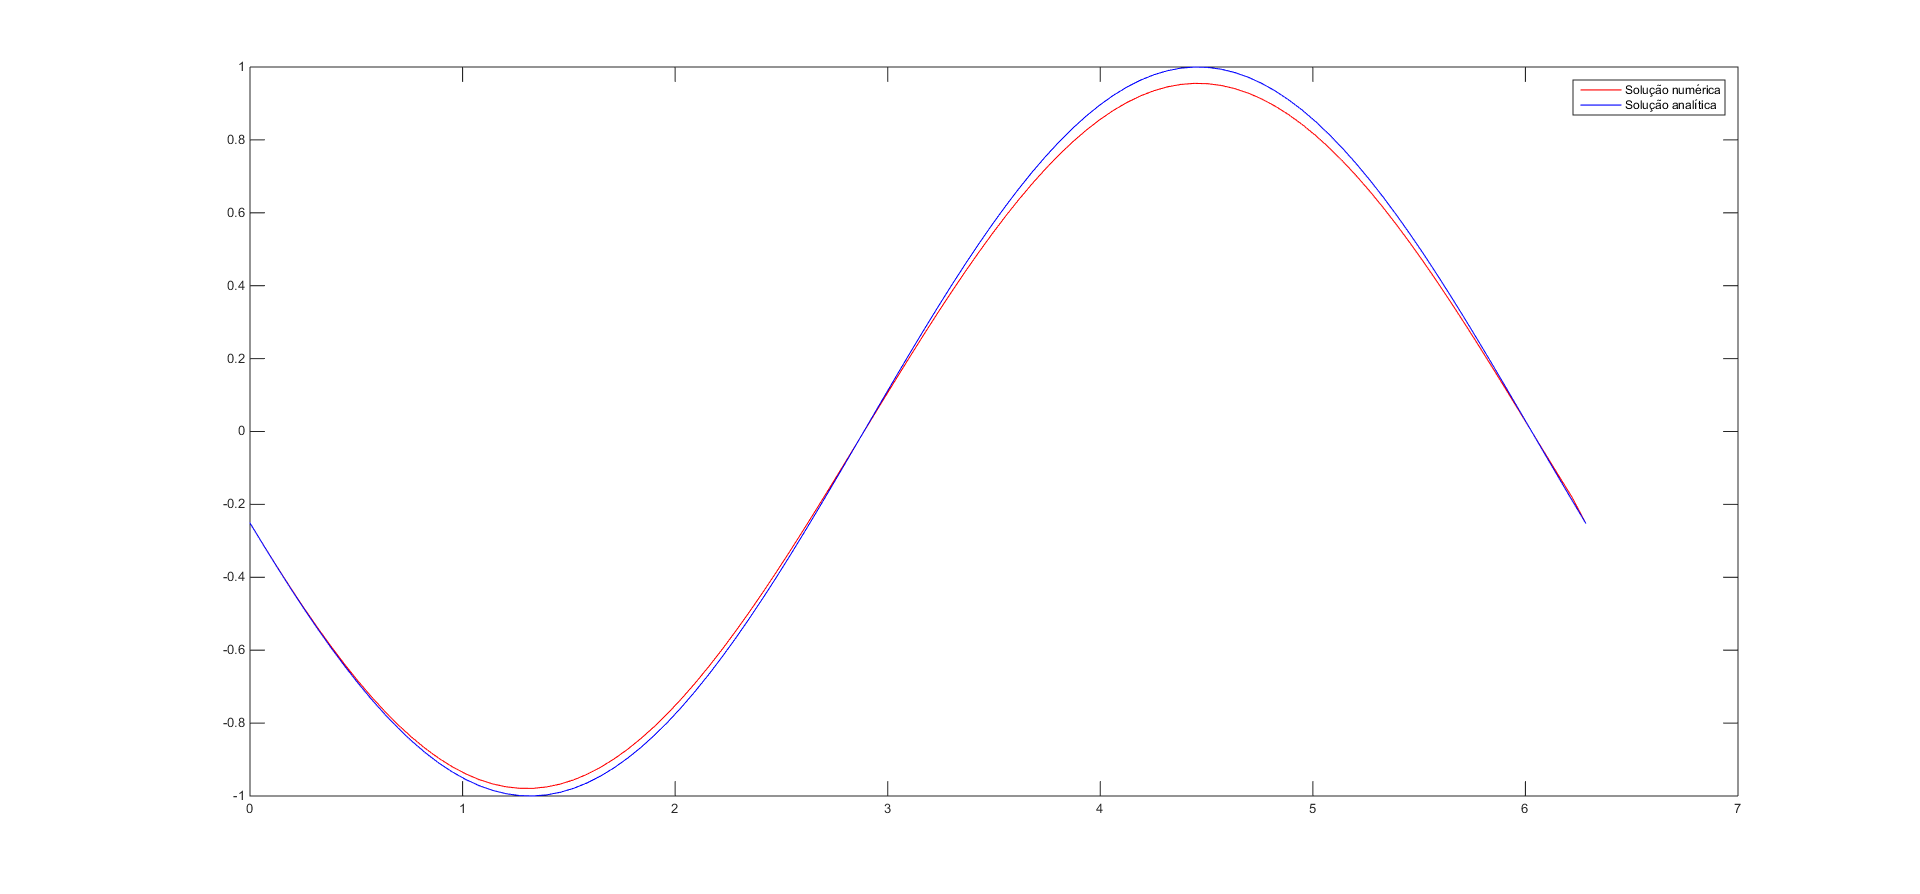
\includegraphics[width=140mm]{Imagens/adveccaouni.png}
	\caption{Advecção unidimensional pelo método explícito}
\end{figure}

	Na Figura(4.6), que fornece o gráfico para o caso de $CFL=1$, observa-se que o erro numérico é tão baixo que as curvas da resolução numérica e analítica se sobrepõem.

\newpage

\begin{figure}[ht!]
	\label{advexplicitoone}
	\centering
	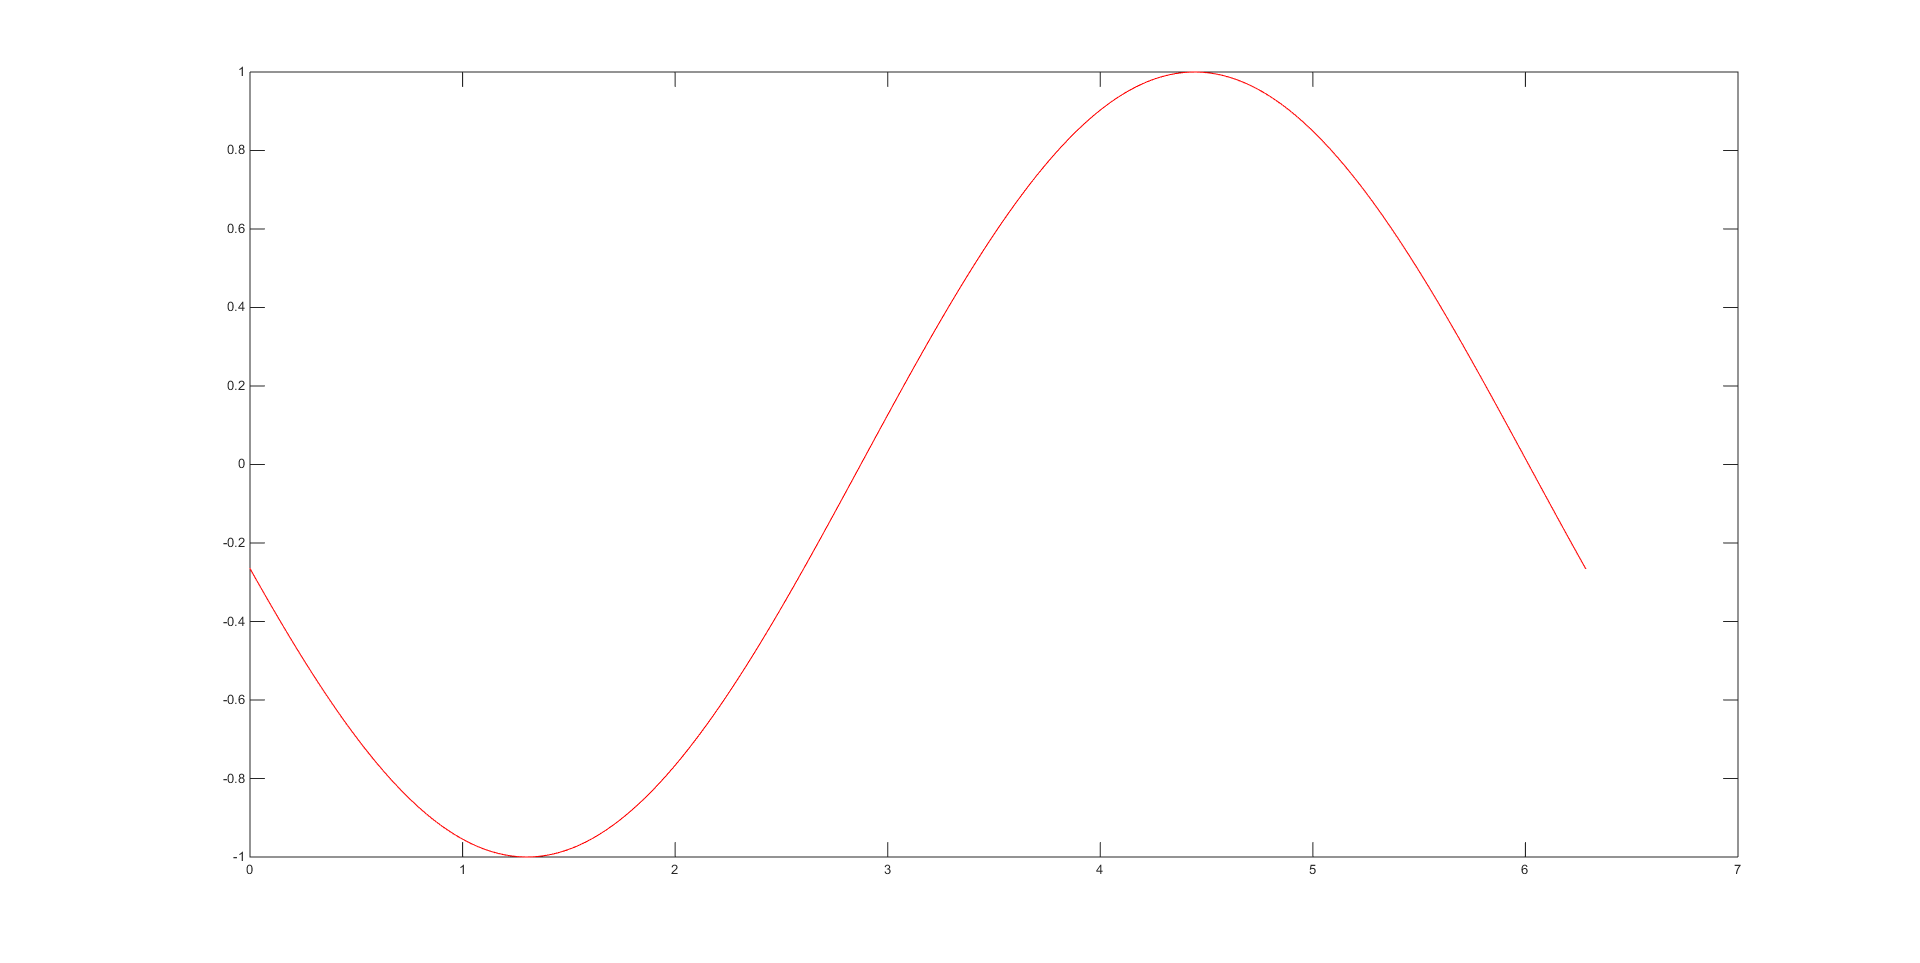
\includegraphics[width=140mm]{Imagens/adveccaounione.png}
	\caption{Advecção unidimensional pelo método explícito com CFL unitário}
\end{figure}	

\section{Advecção Bidimensional}
\noindent

	Os valores obtidos são apresentados na Tabela(\ref{tabela6}). O método continua sendo de primeira ordem para o caso bidimensional. A velocidade de advecção para esse caso é definida como $0,707 \ m/s$, com as velocidades em x e y ($cx \ e\  cy$) definidas como $0,5 \ m/s$.
	
	Novamente é possível observar que nas proximidades do contorno do gráfico, dado em (4.7), que uma grande quantidade de informação é perdida durante a rotina, e essa deficiência é carregada para todo o domínio.
	
	\begin{table}[h!]
	\caption{Erro do método numérico do caso bidimensional explícito para $CFL$=0,8.}
	\label{tabela6}
	\centering
	\begin{tabular}{c | c c c | c c c}
		\hline
		Número de nós  espaciais&       Erro $L_\infty$       	& Razão   	 & Ordem   & Erro $L_{2}$ 				& Razão 	  & Ordem  \\ \hline
		$50$ 					&		$2,70 \, . 10^{-1}$     & $---$      & $---$   &       $9,17 \, . 10^{-2}$  & $---$       & $---$    \\ 
		$100$ 					&       $1,58 \, . 10^{-1}$     & $1,70$     & $0,85$  &       $5,16 \, . 10^{-2}$  & $1,78$      & $0,89$    \\ 
		$200$ 					&       $8,69 \, . 10^{-2}$     & $1,82$     & $0,91$  &       $2,75 \, . 10^{-2}$  & $1,87$      & $0,94$    \\ 
		$400$ 					&       $4,58 \, . 10^{-2}$     & $1,90$     & $0,95$  &       $1,42 \, . 10^{-2}$  & $1,93$      & $0,97$    \\ \hline
%		$800$ 					&       $2,36 \, . 10^{-2}$     & $1,94$     & $0,97$  &       $7,25 \, . 10^{-3}$  & $1,96$      & $0,98$    \\ \hline
	\end{tabular}
\end{table}	

	A comparação da solução numérica com a analítica é dada pela representação gráfica à seguir.

\newpage

\begin{figure}[ht!]
	\label{badvexplicito}
	\centering
	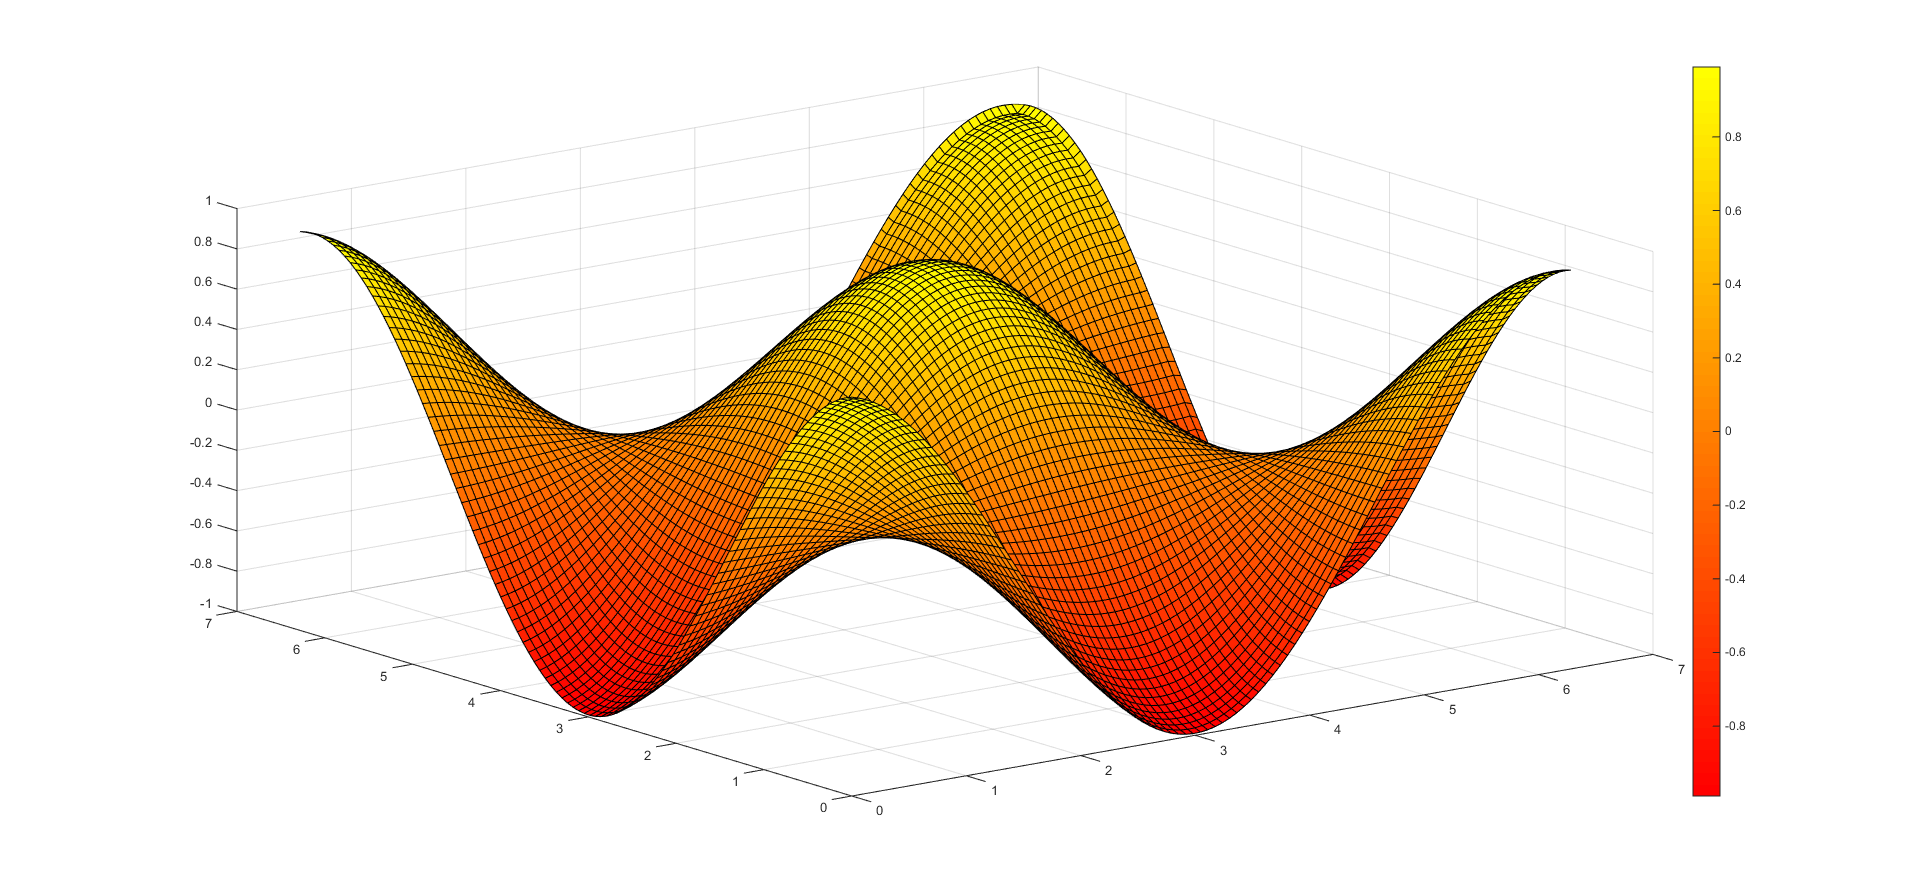
\includegraphics[width=150mm]{Imagens/biadvec.png}
	\caption{Advecção bidimensional pelo método explícito}
\end{figure}
	
\section{Advecção e Difusão Unidimensional}
\noindent

	Trabalha-se agora o efeito conjugado dos mecanismos já avaliados. A Tabela(\ref{tabela7}) fornece os valores obtidos nas simulações para este caso. A velocidade de advecção ($c$) para esse caso é de $1 \ m/s$.
	
	\begin{table}[h!]
	\caption{Erro do método numérico do caso bidimensional explícito para $CFL$=0,8.}
	\label{tabela7}
	\centering
	\begin{tabular}{c | c c c | c c c}
		\hline
		Número de nós  espaciais&       Erro $L_\infty$       	& Razão   	 & Ordem   & Erro $L_{2}$ 				& Razão 	  & Ordem  \\ \hline
		$50$ 					&		$5,08 \, . 10^{-2}$     & $---$      & $---$   &       $3,17 \, . 10^{-2}$  & $---$       & $---$    \\ 
		$100$ 					&       $2,66 \, . 10^{-2}$     & $1,91$     & $0,96$  &       $1,66 \, . 10^{-2}$  & $1,91$      & $0,96$    \\ 
		$200$ 					&       $1,36 \, . 10^{-2}$     & $1,96$     & $0,98$  &       $8,46 \, . 10^{-3}$  & $1,96$      & $0,98$    \\ 
		$400$ 					&       $6,87 \, . 10^{-3}$     & $1,98$     & $0,99$  &       $4,28 \, . 10^{-3}$  & $1,98$      & $0,99$    \\ \hline

	\end{tabular}
\end{table}	

A comparação da solução numérica com a analítica é dada pela Figura(4.8).

\newpage

\begin{figure}[ht!]
	\label{difadvec}
	\centering
	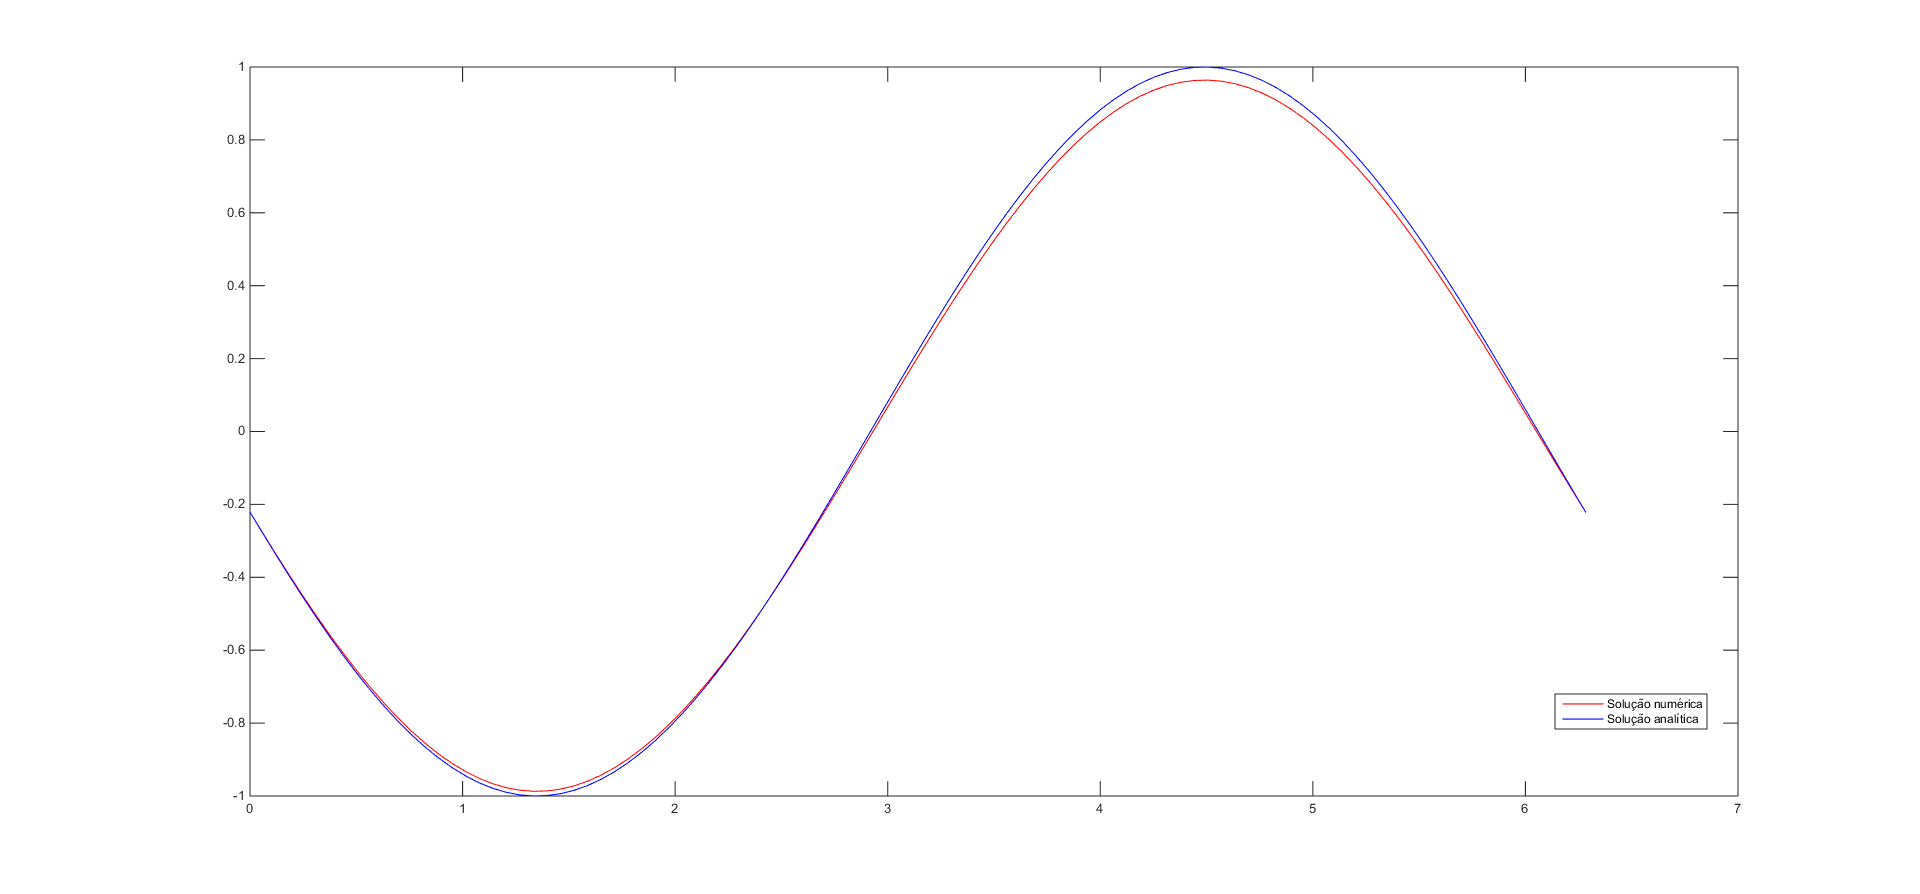
\includegraphics[width=140mm]{Imagens/adveccaoedifusaouni.png}
	\caption{Advecção e difusão unidimensional pelo método explícito}
\end{figure}

\section{Advecção e Difusão Bidimensional}
\noindent

	Finalmente, trabalha-se o efeito conjugado em duas direções. A Tabela(\ref{tabela8}) fornece os valores obtidos nas simulações para este caso. A velocidade na direção x ($cx$) é de $0,8 \ m/s$, enquanto a velocidade na direção y ($cy$) equivale à $0,6 m/s$, resultando numa velocidade de $1 \ m/s$.
	
	\begin{table}[h!]
	\caption{Erro do método numérico do caso bidimensional explícito para $CFL$=0,2.}
	\label{tabela8}
	\centering
	\begin{tabular}{c | c c c | c c c}
		\hline
		Número de nós  espaciais&       Erro $L_\infty$       	& Razão   	 & Ordem   & Erro $L_{2}$ 				& Razão 	  & Ordem  \\ \hline
		$25$ 					&		$9,39 \, . 10^{-2}$     & $---$      & $---$   &       $3,34 \, . 10^{-2}$  & $---$       & $---$    \\ 
		$50$ 					&       $5,03 \, . 10^{-2}$     & $1,87$     & $0,935$  &       $1,83 \, . 10^{-2}$  & $1,83$      & $0,92$    \\ 
		$100$ 					&       $2,60 \, . 10^{-2}$     & $1,93$     & $0,965$  &       $9,57 \, . 10^{-3}$  & $1,91$      & $0,96$    \\ 
		$200$ 					&       $1,32 \, . 10^{-2}$     & $1,97$     & $0,99$  &       $4,89 \, . 10^{-3}$  & $1,96$      & $0,98$    \\ \hline

	\end{tabular}
\end{table}	

A comparação da solução numérica com a analítica é dada pelo gráfico fornecido à seguir.
	
\begin{figure}[ht!]
	\label{bidifadvec}
	\centering
	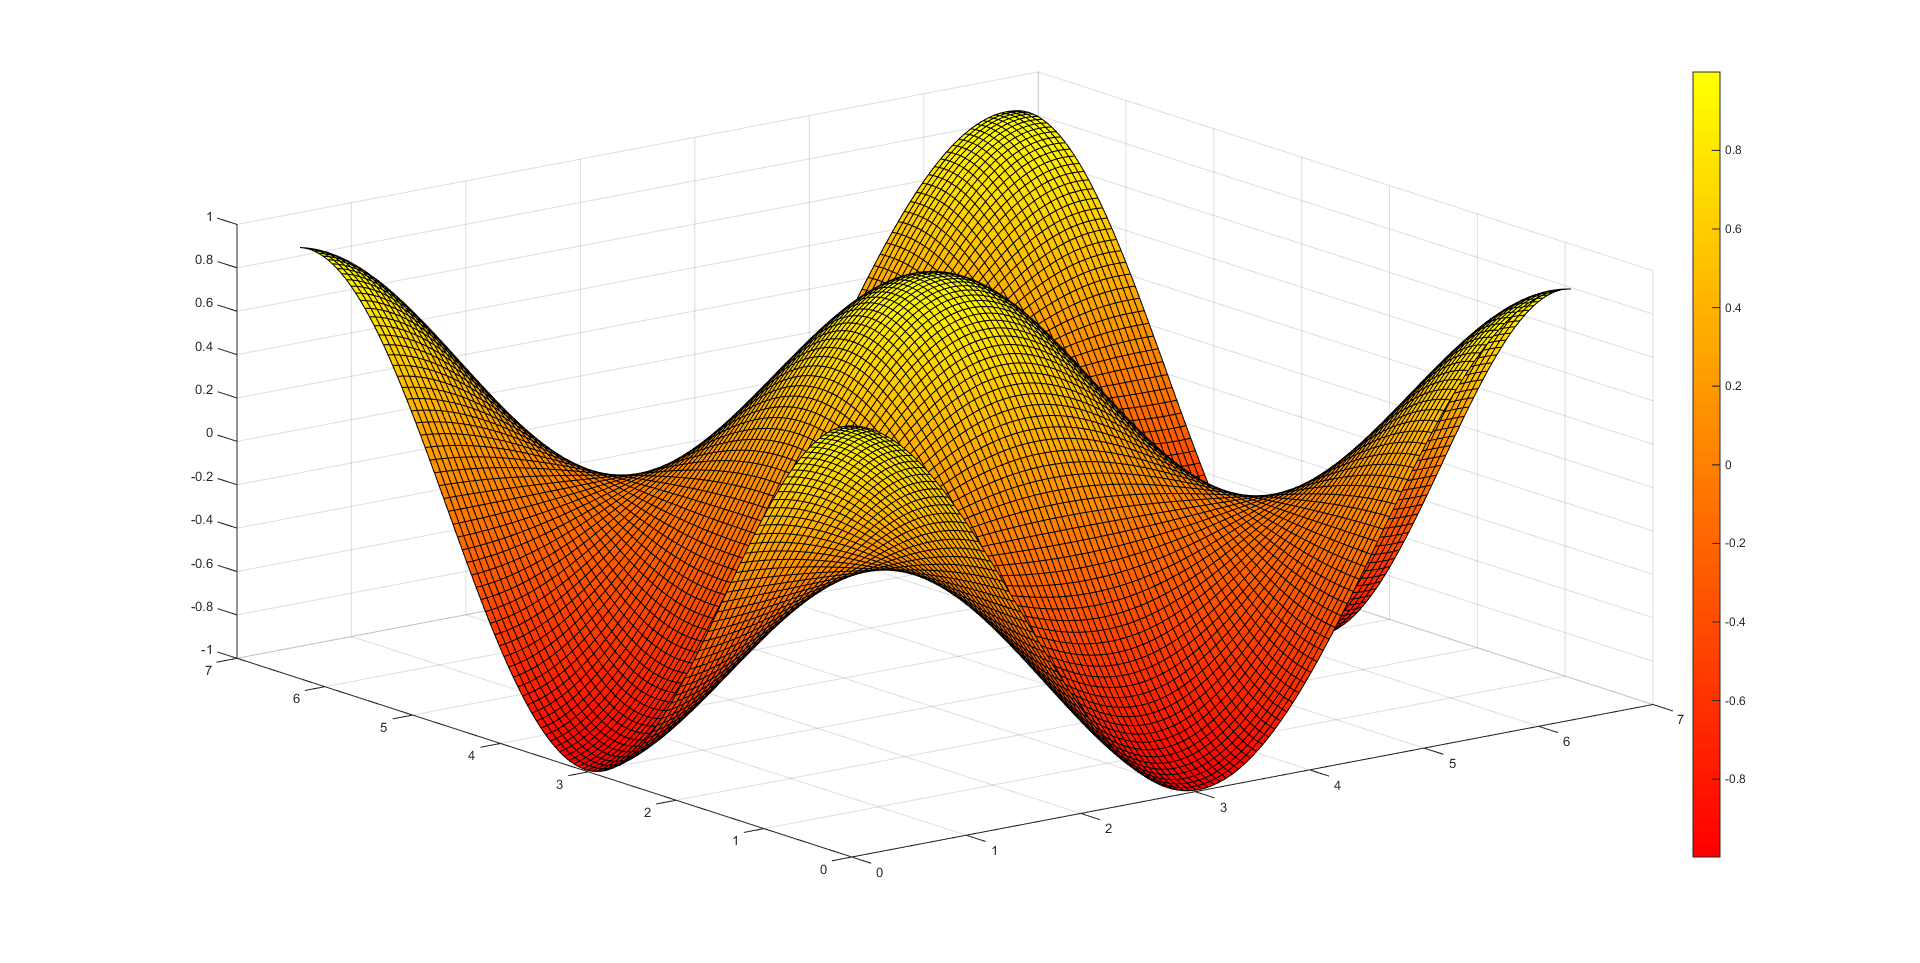
\includegraphics[width=150mm]{Imagens/bidifadvec2.png}
	\caption{Advecção e difusão bidimensional pelo método explícito}
\end{figure}